\documentclass[a4paper]{article}
\usepackage[utf8]{inputenc}
\usepackage{graphicx}
\usepackage{color}
\newcommand{\unam}{\,\mathrm{u}^2}
\newcommand{\una}{\,u$^2$}
\newcommand{\un}{\,u}
\newcommand{\unm}{\,\mathrm{u}}

\newcommand{\len}{\mathrm{length}}
\usepackage{amsmath}
\usepackage{amssymb}
\usepackage{fullpage}
\usepackage[final]{pdfpages}
\title{COMP2911 Project: Preliminary Design} 
\author{Stephen Sherratt, Matthew Todd, Rebecca Wiley}
\begin{document}
\maketitle

\section{Valid moves in Quoridor}

Players take turns to move in Quoridor.
A move is only valid if it occurs on a player's turn.
There are two distinct types of move in Quoridor: 

\begin{itemize}
\item Moving a piece
\item Placing a wall
\end{itemize}

Players must make exactly one move each turn.

    \subsection{Moving a Piece}
    
    A piece may move onto a square directly adjacent to its current square 
        forwards, backwards, left or right unless:
    \begin{itemize}
    \item there is a wall separating the piece's current square from its desired square.
    \item there is no square in the desired direction of travel 
        (ie. the piece is at the edge of the board).
    \end{itemize}
    
    Additionally, if a player's piece is adjacent to their opponent's piece, they
        may move their piece to any square adjacent to the opponent's piece provided that
        it satisfies the two conditions above.

    \subsection{Placing a Wall}

    A wall may be placed in the gaps between squares such that:

    \begin{itemize}
    \item there are two squares on both sides of the wall 
        (ie. it is not on the edge of the board or crossing the edge of the board).
    \item it does not intersect with any walls already placed.
    \item after placing the wall there is at least one path from each player 
        to a square on their respective opposite side of the board.
    \end{itemize}

\pagebreak

\section{Candidate Classes}
    \begin{itemize}
    \item Manager
    \item Game
    \item Move
        \begin{itemize}
        \item MovePiece
        \item PlaceWall
        \end{itemize}
    \item Board
    \item Player
    \item Piece
    \item Wall
    \item Square
    \item Gap
    \end{itemize}


\pagebreak
\section{Class Responsibilities}

\subsection*{Manager}

\begin{tabular}{p{9cm}p{3cm}}
    \textbf{Responsibilities}
    \begin{itemize}
    \item Load Games
    \item Save Games
    \item Create Playels
    \item Start New Game
    \end{itemize}
    &
    \textbf{Collaborators}
    \begin{itemize}
    \item Game
    \item Player
    \end{itemize}
\end{tabular}



\subsection*{Game}

\begin{tabular}{p{9cm}p{3cm}}
    \textbf{Responsibilities}
    \begin{itemize}
    \item Parsing input for moves
    \item Checking validity of moves
    \item Making moves
    \item Undoing and redoing moves
    \item Determining when a game is over
    \end{itemize}
    &
    \textbf{Collaborators}
    \begin{itemize}
    \item Manager
    \item Piece
    \item Wall
    \item Player
    \item Move
    \item Board
    \end{itemize}
\end{tabular}


\subsection*{Move}

\begin{tabular}{p{9cm}p{3cm}}
    \textbf{Responsibilities}
    \begin{itemize}
    \item Describing what type of move is being made
    \item Validating moves
    \end{itemize}
    &
    \textbf{Collaborators}
    \begin{itemize}
    \item Piece
    \item Wall
    \item Player
    \item Board
    \item MovePiece
    \item PlaceWall
    \end{itemize}
\end{tabular}

\subsection*{MovePiece}

\begin{tabular}{p{9cm}p{3cm}}
    \textbf{Responsibilities}
    \begin{itemize}
    \item Describing the movement of a player's piece
    \item Validating movement of a piece
    \end{itemize}
    &
    \textbf{Collaborators}
    \begin{itemize}
    \item Piece
    \item Player
    \item Board
    \item Move
    \end{itemize}
\end{tabular}

\subsection*{PlaceWall}

\begin{tabular}{p{9cm}p{3cm}}
    \textbf{Responsibilities}
    \begin{itemize}
    \item Describing the placement of a wall
    \item Validating placement of a wall
    \end{itemize}
    &
    \textbf{Collaborators}
    \begin{itemize}
    \item Wall
    \item Player
    \item Board
    \item Move
    \end{itemize}
\end{tabular}


\subsection*{Board}

\begin{tabular}{p{9cm}p{3cm}}
    \textbf{Responsibilities}
    \begin{itemize}
    \item Keeping track of wall locations
    \item Checking for paths players can take
    \item Formatting output so board can be displayed
    \end{itemize}
    &
    \textbf{Collaborators}
    \begin{itemize}
    \item Wall
    \item Piece
    \item Square
    \item Gap
    \end{itemize}
\end{tabular}


\subsection*{Player}

\begin{tabular}{p{9cm}p{3cm}}
    \textbf{Responsibilities}
    \begin{itemize}
    \item Keep track of how many walls a player has left
    \item Store the player's name
    \item Keep track of the player's piece
    \end{itemize}
    &
    \textbf{Collaborators}
    \begin{itemize}
    \item Piece
    \end{itemize}
\end{tabular}

\subsection*{Piece}

\begin{tabular}{p{9cm}p{3cm}}
    \textbf{Responsibilities}
    \begin{itemize}
    \item Keep track of a piece's position
    \item Move a piece
    \end{itemize}
    &
    \textbf{Collaborators}
    \begin{itemize}
    \item Square
    \end{itemize}
\end{tabular}



\subsection*{Wall}
\begin{tabular}{p{9cm}p{3cm}}
    \textbf{Responsibilities}
    \begin{itemize}
    \item Keep track of wall's position
    \item Be created in desired position
    \end{itemize}
    &
    \textbf{Collaborators}
    \begin{itemize}
    \item Gap
    \end{itemize}
\end{tabular}



\subsection*{Square}
\begin{tabular}{p{9cm}p{3cm}}
    \textbf{Responsibilities}
    \begin{itemize}
    \item Have coordinates
    \end{itemize}
    &
    \textbf{Collaborators}
\end{tabular}

\subsection*{Gap}
\begin{tabular}{p{9cm}p{3cm}}
    \textbf{Responsibilities}
    \begin{itemize}
    \item Have coordinates
    \item Keep track of whether or not there is a wall in the gap
    \item Know which wall is in the gap (if any)
    \end{itemize}
    &
    \textbf{Collaborators}

    \begin{itemize}
    \item Wall
    \end{itemize}
\end{tabular}

\pagebreak

\section{Class Diagram}

\begin{tabular}{p{12cm}}
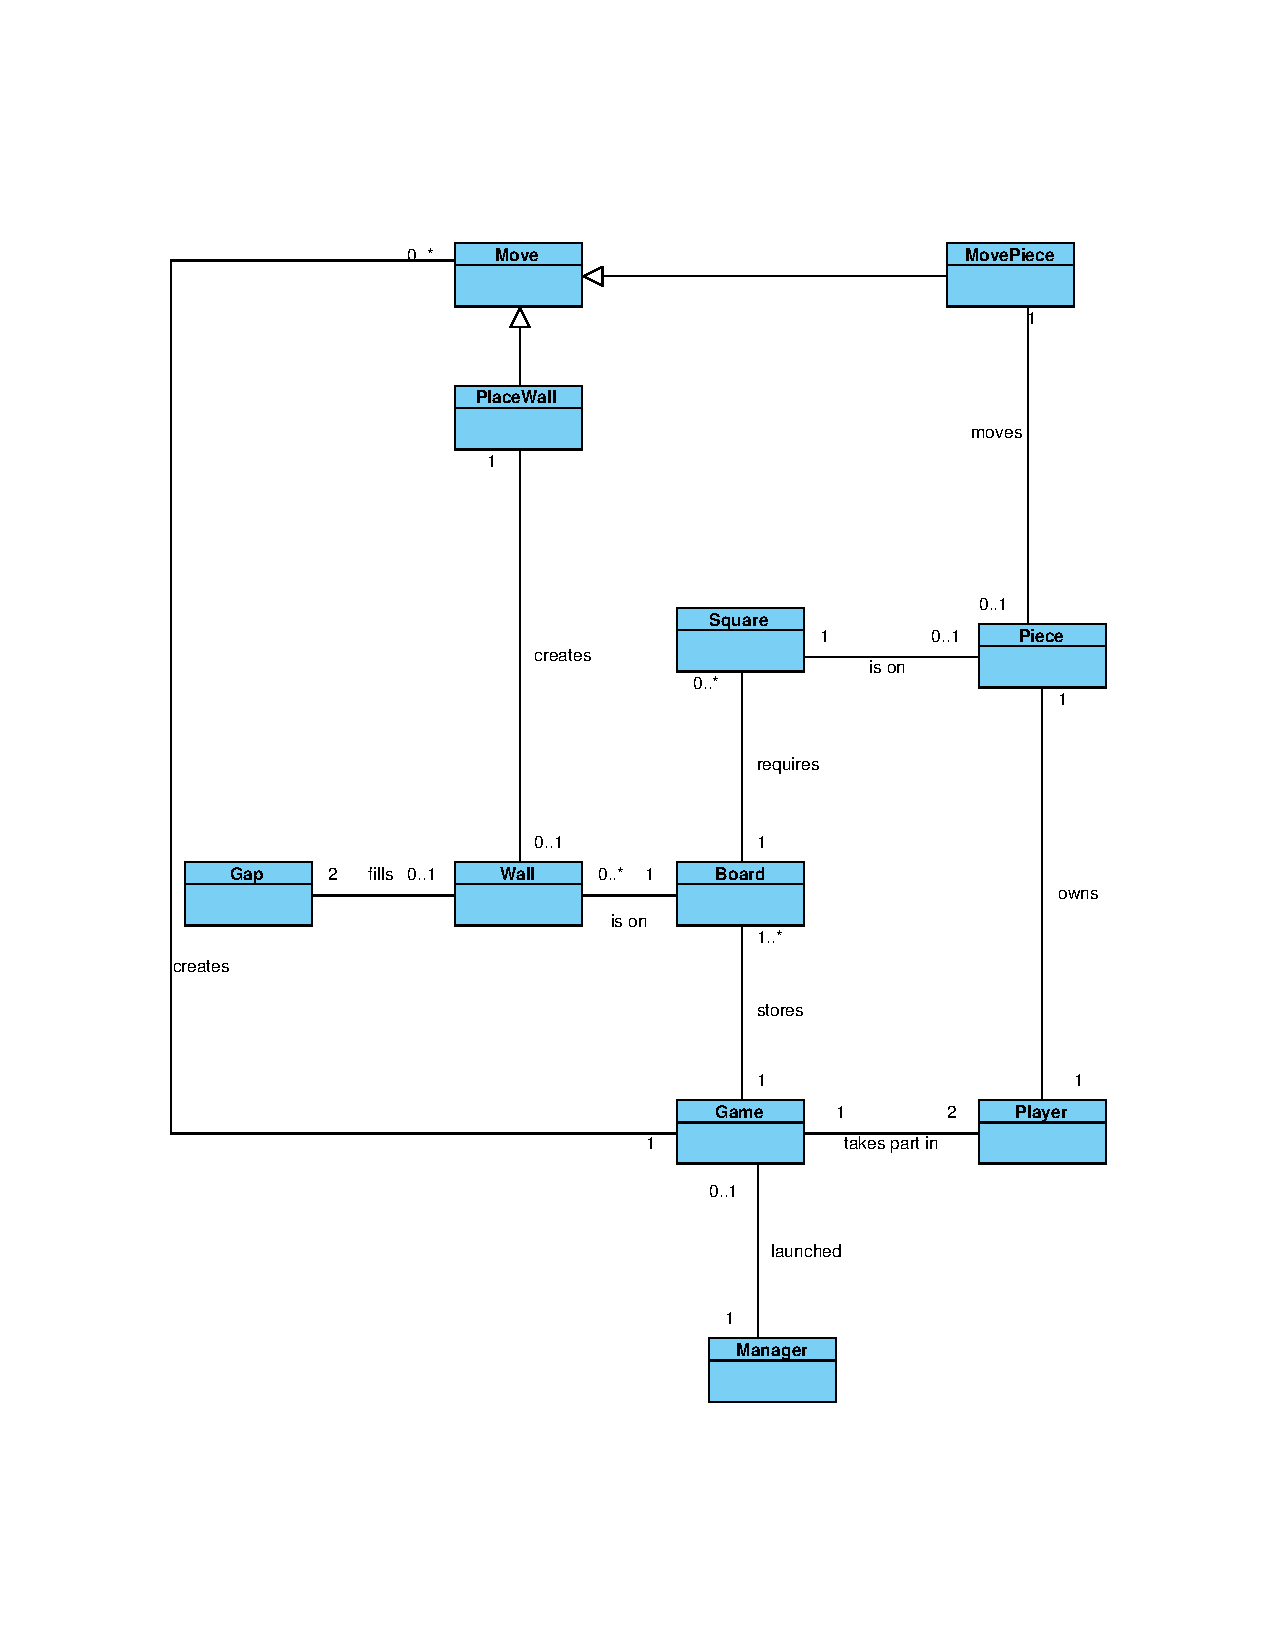
\includepdf[scale=1]{classdiagram.pdf}
\end{tabular}

\end{document}
